\begin{solution}
    \textbf{a.} \textbf{证明:}

    (1)唯一的最小生成树:\\
    \qquad 采用反证法。假设最小生成树不唯一,则存在两棵最小生成树$T_1$和$T_2$,满足$w(T_1)=w(T_2)$,
    由于图中所有的边权重均不相等,故可以约定边$e$是$(T_1\cup T_2) - (T_1 \cap T_2)$中唯一最大的。不失一般性地,假设$e$来自于$T_1$,
    即$e\in T_1 \wedge e\notin T_2$。若在$T_1$中$e$连接的两个连通分量为$C_1$,$C_2$,那么在$T_2$中
    必然至少存在另一条边$e'$连接了$C_1$,$C_2$,且因为$e$是唯一最大的,$w(e)>w(e')$,此时
    $T'_1 = T_1 - \{e\}\cup \{e'\}$显然仍是$G$的最小生成树,且$w(T'_1)<w(T_1)$,即可以找到更优的最小
    生成树$T'_1$。故假设不成立,即图$G$有唯一的最小生成树。

    (2)可能不唯一的次优最小生成树:\\
    \qquad 采用构造法。图$G$如下图所示:
    \begin{center}
        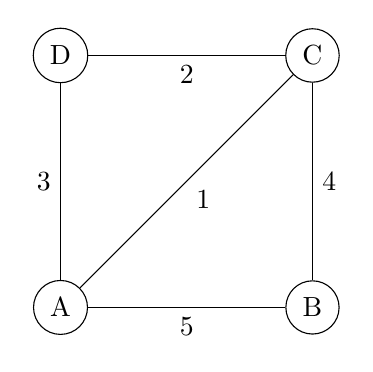
\begin{tikzpicture}
            \begin{scope}[scale=.8,auto=left,every node/.style={circle,draw=black}]
            \node (A) at (0,0)  {A};
            \node (B) at (4,0)  {B};
            \node (C) at (4,4)  {C};
            \node (D) at (0,4)  {D};
            \end{scope}
            \path (A) edge [below] node {$5$} (B);
            \path (B) edge [right] node {$4$} (C);
            \path (C) edge [below] node {$2$} (D);
            \path (A) edge [left] node {$3$} (D);
            \path (A) edge [below right] node {$1$} (C);
        \end{tikzpicture}
    \end{center}
    它的最小生成树总代价为7:
    \begin{center}
        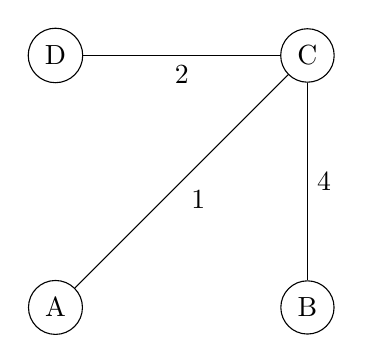
\begin{tikzpicture}
            \begin{scope}[scale=.8,auto=left,every node/.style={circle,draw=black}]
            \node (A) at (0,0)  {A};
            \node (B) at (4,0)  {B};
            \node (C) at (4,4)  {C};
            \node (D) at (0,4)  {D};
            \end{scope}
            % \path (A) edge [below] node {$5$} (B);
            \path (B) edge [right] node {$4$} (C);
            \path (C) edge [below] node {$2$} (D);
            % \path (A) edge [left] node {$3$} (D);
            \path (A) edge [below right] node {$1$} (C);
        \end{tikzpicture}
    \end{center}
    然而,它有两棵总代价为8的次优最小生成树:
    \begin{figure}[htbp]
        \begin{minipage}[t]{0.48\textwidth}\centering
            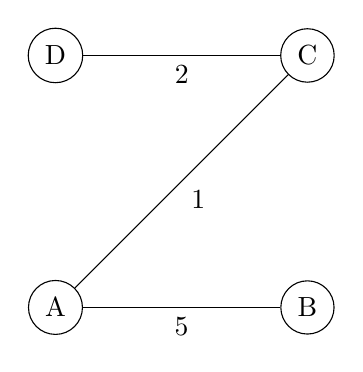
\begin{tikzpicture}
                \begin{scope}[scale=.8,auto=left,every node/.style={circle,draw=black}]
                \node (A) at (0,0)  {A};
                \node (B) at (4,0)  {B};
                \node (C) at (4,4)  {C};
                \node (D) at (0,4)  {D};
                \end{scope}
                \path (A) edge [below] node {$5$} (B);
                \path (C) edge [below] node {$2$} (D);
                \path (A) edge [below right] node {$1$} (C);
            \end{tikzpicture}
        \end{minipage}
        \begin{minipage}[t]{0.48\textwidth}\centering
            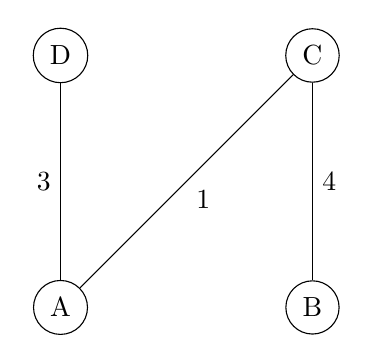
\begin{tikzpicture}
                \begin{scope}[scale=.8,auto=left,every node/.style={circle,draw=black}]
                \node (A) at (0,0)  {A};
                \node (B) at (4,0)  {B};
                \node (C) at (4,4)  {C};
                \node (D) at (0,4)  {D};
                \end{scope}
                \path (B) edge [right] node {$4$} (C);
                \path (A) edge [left] node {$3$} (D);
                \path (A) edge [below right] node {$1$} (C);
            \end{tikzpicture}
        \end{minipage}
    \end{figure}

    \textbf{b.} \textbf{证明:}\\
    \textit{引理:}若$T$是图$G$的一棵生成树,对于$G$中边构成的集合$A$、$B$,满足$A \subseteq T \wedge A\cap B = \emptyset$,
    若$T' = T-A\cup B$亦是图$G$的一棵生成树,则对任意边$p\in A$,总存在边$p'\in B$,使得$T-\{p\}\cup \{p'\}$是生成树。

    引理的证明:采用反证法。若存在边$p\in A$,其连接的两个连通分量为$C_1$、$C_2$,如果
    对任意$p'\in B$,使得$T-\{p\}\cup \{p'\}$不是生成树,则说明对于任意$p'\in B$不能够连接$C_1$、$C_2$两个
    连通分量。于是$T-\{p\}\cup B$不能连接$C_1$、$C_2$两个连通分量,即它是非连通图。而非连通图去除一些边之后的子图也
    一定是非连通图,即$T' = T-A\cup B$是非连通的,而$T'$是生成树,一定是连通的,产生矛盾,引理得证。

    下面利用上面的引理进行证明。\\
    假设图$G$的一棵次优最小生成树为$T'=T-A\cup B$,其中$T$是图$G$的最小生成树。
    假设对于任意某个$s\in A$,根据引理可得,一定存在$s'\in B$,$T''=T-\{s\}\cup \{s'\}$亦是图$G$的生成树,由于$T$是图$G$
    唯一的最小生成树(在\textbf{a}中已经证明),故得到$w(T'')>w(T)$,进而$w(s')>w(s)$。将所有$s\in A$对应$s'$构成的集合记作$A'$,
    则显然有$A'\subseteq B$,假设$t$满足$t\in A' \wedge w(t) = \max_{i \in A'} w(i)$,那么$t$一定满足
    $t \in B \wedge \forall s \in A, w(t)>w(s)$。\\
    另一方面,显然还存在这样的逆向替换即$T=T'-B\cup A$,此时对于$t \in B$,再次利用引理,则一定存在$t' \in A$,
    $T'''=T'-\{t\}\cup \{t'\}$亦是$G$的生成树。此时,$w(T''') = w(T') - w(t) + w(t')$。上一段落已证明了$w(t)>w(t')$,于是
    $w(T''') < w(T')$。这说明了,对于任意的一棵非最小生成树的生成树,一定存在仅改变一条边的变换使得生成树的代价更小。因此
    次优最小生成树一定是$T-\{(u,v)\}\cup\{(x,y)\}$的形式。

    \textbf{c.}\\
    \textbf{d.}\\
\end{solution}